\documentclass[12pt]{article}

\usepackage[margin=1in]{geometry}
\usepackage[T1]{fontenc}
\usepackage{lmodern}
\usepackage{microtype}
\usepackage{amsmath,amssymb,mathtools}
\usepackage{booktabs}
\usepackage{enumitem}
\usepackage{setspace}
\usepackage{xcolor}
\usepackage{tikz}
\usepackage{hyperref}
\usepackage{xurl}

\hypersetup{
  colorlinks=true,
  linkcolor=black,
  citecolor=black,
  urlcolor=blue,
  pdftitle={Is the Galaxy Acceleration Scale Cosmic?},
  pdfauthor={Light-Meter Physics},
  pdfsubject={The empirical radial acceleration relation and conditional links to cosmological scales},
  pdfkeywords={radial acceleration relation, galaxy dynamics, cosmological acceleration, entropy model, horizon scale}
}

\onehalfspacing
\widowpenalty=10000
\clubpenalty=10000
\definecolor{ink}{HTML}{172E3D}
\definecolor{teal}{HTML}{126D77}
\definecolor{rust}{HTML}{B1533E}
\definecolor{violet}{HTML}{796493}

\title{Is the Galaxy Acceleration Scale Cosmic?\\
Evidence, a Conditional Model, and Open Tests}
\author{Light-Meter Physics}
\date{}

\begin{document}

\maketitle

\begin{abstract}
Disk galaxies exhibit a tight empirical relation between the Newtonian acceleration calculated from their observed baryons and the radial acceleration inferred from their rotation curves. The characteristic acceleration in a widely used fit is numerically close to several combinations of the present Hubble scale. This manuscript asks whether that proximity has a physical explanation, while keeping observation, dimensional coincidence, model assumption, and conditional consequence distinct. It derives the time-scale identities used in the proposed argument and follows an entropy-based construction to a spherical response estimate. Within that model, the response scale, the equal-entropy boundary, and the measured galaxy scale are different quantities, even when their numerical values are similar. The unsuppressed response conflicts with Solar-System constraints, and an observationally viable high-acceleration suppression has not been derived. Horizon-scale comparisons depend on a specified cosmological background; translating them into galaxy-scale evolution requires an additional coupling and response-history prescription. The result is a critical account of a speculative proposal, not a derivation of a new law of gravity or evidence that the radial acceleration relation has a unique cause.
\end{abstract}

\noindent\textbf{Keywords:} radial acceleration relation, galaxy dynamics, cosmological acceleration, entropy model, horizon scale

\section{Introduction}
\label{sec:introduction}

Rotationally supported galaxies show a close relation between the gravitational acceleration expected from their baryonic matter and the radial acceleration inferred from their rotation curves. The empirical relation is often summarized by a characteristic acceleration $a_0$ of order $10^{-10}\,\mathrm{m\,s^{-2}}$ \cite{McGaughRAR}. The value is also close, within order-unity factors, to accelerations constructed from the Hubble parameter and the speed of light. That numerical proximity is interesting, but by itself it does not establish a causal connection between galaxy dynamics and cosmic expansion.

The purpose here is to distinguish the observed RAR, exact identities within spherical Newtonian bookkeeping, assumptions in the entropy-response model, and unresolved physical claims. The question is whether a cosmic-scale connection can be derived and tested across galaxies, the Solar System, lensing, and other low-acceleration systems. The algebra follows conditionally, but the physical coupling, an observationally viable high-acceleration suppression, and a unique cosmological scale remain open.

The manuscript first describes the measured RAR and its limits. It then compares the empirical scale with several distinct combinations of $H_0$, derives the time-scale identities, and reconstructs the entropy-based spherical estimate. A final comparison addresses the failures and tests that any complete theory must resolve.

\section{The empirical radial acceleration relation}
\label{sec:rar}

For a galaxy with circular speed $V_c(r)$ at radius $r$, define the observed radial acceleration by
\begin{equation}
  g_{\rm obs}(r)\equiv\frac{V_c^2(r)}{r}.
  \label{eq:g-observed}
\end{equation}
This is a coordinate acceleration associated with circular motion in the adopted galactic model. It is not, in general, the proper acceleration of a star moving on a freely falling orbit. Let $g_B(r)$ denote the Newtonian radial acceleration calculated from the observed baryonic mass distribution, including stars and gas. In a spherical approximation with enclosed baryonic mass $M_B(r)$,
\begin{equation}
  g_B(r)=\frac{G M_B(r)}{r^2}.
  \label{eq:g-baryon}
\end{equation}
For flattened disks, $g_B$ is calculated from the disk geometry rather than this spherical expression.

The original RAR study found that these quantities follow a tight empirical trend across its galaxy sample and represented it with the fit
\begin{equation}
  \begin{aligned}
    g_{\rm obs}
    &=\frac{g_B}{1-\exp\!\left[-\sqrt{g_B/a_0}\right]},\\
    a_0&=(1.20\pm0.02_{\rm random}\pm0.24_{\rm systematic})
      \times10^{-10}\,\mathrm{m\,s^{-2}}.
  \end{aligned}
  \label{eq:rar-fit}
\end{equation}
The random uncertainty is quoted at $1\sigma$; the systematic term reflects the adopted stellar mass-to-light normalization. They are reported separately and are not combined here as independent statistical errors \cite{McGaughRAR}. Equation~\eqref{eq:rar-fit} is a fitting function for the data; it is not by itself a microscopic theory or a uniquely identified force law.

In the high-acceleration limit, $g_B/a_0\gg1$, the exponential term tends to zero and $g_{\rm obs}\simeq g_B$. In the low-acceleration limit, $g_B/a_0\ll1$, expansion of the exponential gives
\begin{equation}
  1-\exp\!\left[-\sqrt{g_B/a_0}\right]
  \simeq\sqrt{g_B/a_0},
  \qquad
  g_{\rm obs}\simeq\sqrt{a_0g_B}.
  \label{eq:rar-limits}
\end{equation}
For an idealized outer orbit around a concentrated baryonic mass, use $g_B\simeq GM_B/r^2$ and $g_{\rm obs}\simeq V_c^2/r$. If the low-acceleration approximation applies, then
\begin{equation}
  \frac{V_c^2}{r}\simeq\frac{\sqrt{GM_Ba_0}}{r},
  \qquad
  V_c^4\simeq GM_Ba_0.
  \label{eq:btfr-limit}
\end{equation}
This familiar scaling follows here only under the stated outer-orbit and concentrated-mass assumptions. It does not establish the physical origin of $a_0$.

\begin{figure}[ht]
  \centering
  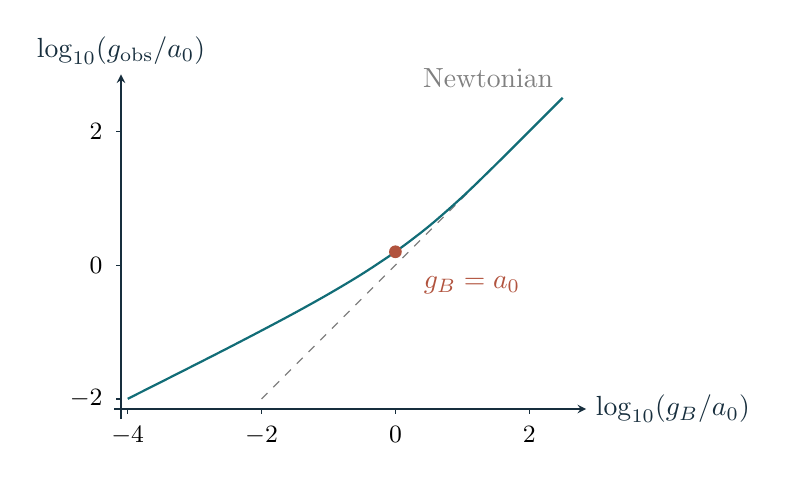
\begin{tikzpicture}[x=0.85cm,y=0.85cm,>=stealth]
    \draw[->,ink] (-4.2,-2.15)--(2.85,-2.15)
      node[right] {$\log_{10}(g_B/a_0)$};
    \draw[->,ink] (-4.1,-2.3)--(-4.1,2.85)
      node[above] {$\log_{10}(g_{\rm obs}/a_0)$};
    \foreach \x in {-4,-2,0,2}{
      \draw[ink] (\x,-2.15)--(\x,-2.23);
      \node[anchor=north,font=\small] at (\x,-2.26) {$\x$};
    }
    \foreach \y in {-2,0,2}{
      \draw[ink] (-4.1,\y)--(-4.18,\y);
      \node[anchor=east,font=\small] at (-4.23,\y) {$\y$};
    }
    \draw[dashed,gray] (-2,-2)--(2.5,2.5)
      node[above left,text=gray] {Newtonian};
    \draw[thick,teal,smooth] plot coordinates {
      (-4,-1.998) (-3.5,-1.746) (-3,-1.493) (-2.5,-1.238)
      (-2,-0.978) (-1.5,-0.712) (-1,-0.433) (-0.5,-0.134)
      (0,0.199) (0.5,0.580) (1,1.019) (1.5,1.502)
      (2,2.000) (2.5,2.500)
    };
    \fill[rust] (0,0.199) circle (2.3pt);
    \node[anchor=west,rust] at (0.28,-0.30) {$g_B=a_0$};
  \end{tikzpicture}
  \caption{The analytic curve from Eq.~\eqref{eq:rar-fit} in logarithmic coordinates, together with the Newtonian line. This is a plot of the published fitting form, not a reproduction of individual galaxy measurements.}
  \label{fig:rar-fit}
\end{figure}

The empirical relation leaves open how the trend arises. Baryonic mass modeling, sample selection, galaxy structure, and residual correlations matter to its interpretation. Competing accounts can reproduce or seek to explain parts of the relation; the fit alone does not select among them. In particular, agreement with Eq.~\eqref{eq:rar-fit} in one regime does not show that a proposed cosmic mechanism also satisfies high-acceleration constraints or predicts light bending.

\section{Several different acceleration scales}
\label{sec:scales}

To compare $a_0$ with cosmic scales, adopt as a reference the flat matter-plus-$\Lambda$ cosmology used for the numerical examples,
\begin{equation}
  H_0=67.4\,\mathrm{km\,s^{-1}\,Mpc^{-1}},
  \qquad
  \Omega_m=0.315,
  \qquad
  \Omega_\Lambda=0.685,
  \label{eq:cosmo-inputs}
\end{equation}
with radiation neglected for the background calculations \cite{Planck}. These are specified inputs, not a claim that the Hubble constant is known without measurement-method dependence. For example, the 2022 SH0ES Cepheid--supernova distance-ladder analysis reports $H_0=73.04\pm1.04\,\mathrm{km\,s^{-1}\,Mpc^{-1}}$ \cite{Riess}. Substituting that central value into $cH_0/(2\pi)$ gives $1.13\times10^{-10}\,\mathrm{m\,s^{-2}}$, about $8.4\%$ above the value from the reference $H_0$. This comparison illustrates dependence on the adopted measurement; it does not resolve the differing determinations or select a unique $H_0$.

For the reference inputs, the following quantities are numerically near one another in some cases, but they have different definitions and roles:
\begin{table}[ht]
  \centering
  \small
  \begin{tabular}{@{}lll@{}}
    \toprule
    Quantity & Value ($\mathrm{m\,s^{-2}}$) & Status in this manuscript \\
    \midrule
    $a_0$ & $1.20\times10^{-10}$ & Empirical RAR fit scale \\
    $cH_0/(2\pi)$ & $1.04\times10^{-10}$ & Numerical comparison \\
    $a_M=cH_0/6$ & $1.09\times10^{-10}$ & Model response normalization \\
    $cH_0/2$ & $3.27\times10^{-10}$ & Entropy-model crossover \\
    $cH_\Lambda$ & $5.42\times10^{-10}$ & Fixed-$\Lambda$ candidate scale \\
    $cH_0$ & $6.55\times10^{-10}$ & Hubble acceleration scale \\
    \bottomrule
  \end{tabular}
  \caption{Distinct acceleration scales evaluated with Eqs.~\eqref{eq:cosmo-inputs} and $H_\Lambda=H_0\sqrt{\Omega_\Lambda}$. The values are rounded. Similar magnitudes do not make the definitions equivalent.}
  \label{tab:acceleration-scales}
\end{table}

The same comparison can be expressed in inverse-time units:
\begin{equation}
  \frac{a_0}{c}\simeq4.00\times10^{-19}\,\mathrm{s^{-1}},
  \qquad
  \frac{H_0}{2\pi}\simeq3.48\times10^{-19}\,\mathrm{s^{-1}}.
  \label{eq:rate-coincidence}
\end{equation}
For the adopted $H_0$, the ratio $a_0/[cH_0/(2\pi)]$ is about $1.15$. Using the displayed central values, $cH_0/(2\pi)$ is about $13\%$ below $a_0$, while the quoted systematic uncertainty is about $20\%$ of the central $a_0$. This is not a significance test: the systematic term is not treated here as an independent statistical error. The factor $2\pi$ is an approximate numerical coefficient in this comparison, not a derivation from a periodic process: $H_0$ has units of inverse time and is not itself a cycle frequency. The times $c/a_0\simeq79.2\,\mathrm{Gyr}$ and $2\pi/H_0\simeq91.2\,\mathrm{Gyr}$ restate the same approximate comparison.

The table is deliberately explicit about the differences between $a_0$, $cH_0/(2\pi)$, the model's $a_M=cH_0/6$, and the entropy boundary $cH_0/2$. The latter two arise from distinct steps in the proposed construction. Their proximity to $a_0$ is suggestive only if a theory derives the relevant coefficients and survives independent tests. A dimensional coincidence does not by itself provide that theory.

\section{Gravitational time, radial light time, and compactness}
\label{sec:identities}

In the spherical Newtonian bookkeeping model, let $M_B(r)$ be the baryonic mass enclosed within radius $r$. Define the gravitational time, radial light-travel time, and Hubble time by
\begin{equation}
  \tau_g\equiv\frac{GM_B}{c^3},
  \qquad
  t_r\equiv\frac{r}{c},
  \qquad
  t_H\equiv\frac{1}{H}.
  \label{eq:times}
\end{equation}
With $g_B=GM_B/r^2$, direct substitution gives
\begin{equation}
  \frac{g_B}{c}=\frac{\tau_g}{t_r^2},
  \qquad
  x_R\equiv\frac{GM_B}{rc^2}=\frac{\tau_g}{t_r}.
  \label{eq:time-identities}
\end{equation}
These are unit-consistent rewritings of the spherical Newtonian acceleration and compactness. They do not introduce a new frequency or show that the Hubble expansion acts on a bound system.

The first identity is sometimes described as expressing acceleration in inverse-time units, since $g_B/c$ has units $\mathrm{s^{-1}}$. It should not be called an oscillation frequency without a specified periodic process. Likewise, $x_R$ is a compactness parameter, not a general clock-rate field. In the Schwarzschild exterior, a static clock has $dt/d\tau=(1-2x_R)^{-1/2}\simeq1+x_R$ only in the weak-field limit. A compactness ratio or a first-order clock-rate excess cannot be transferred unchanged to a general cosmological setting.

\section{The entropy construction: where assumptions enter}
\label{sec:entropy-model}

An entropy-based proposal introduces a model quantity $S_M$ for the magnitude of an entropy displacement associated with baryonic matter, and compares it with an area entropy. In the construction considered here,
\begin{equation}
  |S_M|\equiv\frac{2\pi k_B M_B c r}{\hbar},
  \qquad
  S_A\equiv\frac{k_B A}{4\ell_P^2},
  \qquad
  A=4\pi r^2,
  \qquad
  \ell_P^2=\frac{\hbar G}{c^3}.
  \label{eq:entropy-definitions}
\end{equation}
Substitution yields
\begin{equation}
  \frac{|S_M|}{S_A}
  =\frac{2GM_B}{rc^2}=2x_R.
  \label{eq:entropy-compactness}
\end{equation}
Equation~\eqref{eq:entropy-compactness} is exact algebra given the definitions in Eq.~\eqref{eq:entropy-definitions}. It does not independently establish that $S_M$ is a thermodynamic entropy; here it is a model's displacement magnitude \cite{Verlinde}.

For a generic radius-$r$ sphere, $S_A$ is a horizon-inspired reference entropy in this construction, not an independently measured entropy of that galactic surface. The horizon area law alone does not establish this assignment for every sphere.

The next step is an additional hypothesis: assign a volume entropy $S_V$ proportional to the area entropy and to the ratio of radius to a de Sitter horizon scale $L=c/H$,
\begin{equation}
  S_V\equiv\frac{r}{L}S_A=\frac{t_r}{t_H}S_A.
  \label{eq:volume-entropy}
\end{equation}
Here $H$ is the constant expansion rate of the assumed de Sitter background. For the illustrative numerical normalization below, we identify this model rate with today's $H_0$; that calibration is not derived from the entropy assignments. Replacing $H$ with a time-dependent $H(t)$ in an evolving cosmology is a further hypothesis, not a consequence of this construction. The volume-entropy prescription itself is not implied by the area-entropy formula. Defining $\epsilon_M\equiv|S_M|/S_V$, the assumed relations give
\begin{equation}
  \epsilon_M
  =\frac{2\tau_g t_H}{t_r^2}
  =\frac{2g_B}{cH}.
  \label{eq:epsilon-m}
\end{equation}
If equal contributions are identified with $\epsilon_M=1$, the model's crossover criterion is
\begin{equation}
  g_{B,\mathrm{cross}}=\frac{cH}{2}.
  \label{eq:entropy-crossover}
\end{equation}
This is a conditional consequence of Eq.~\eqref{eq:volume-entropy} and the equality criterion, not a measured threshold or a universal boundary between two established laws.

The same model-defined crossover can be expressed as a radius and a light-travel-time scale:
\begin{equation}
  r_{\rm cross}^2=\frac{2G M_B(r_{\rm cross})}{cH},
  \qquad
  t_{\rm cross}\equiv\frac{r_{\rm cross}}{c}
  =\sqrt{2\tau_g(r_{\rm cross})t_H}.
  \label{eq:crossover-scales}
\end{equation}
For a concentrated mass this gives an explicit radius; for an extended profile the enclosed mass is evaluated at the unknown crossover radius, so the relation is implicit. The quantity $t_{\rm cross}$ is a length expressed in light-travel-time units, not a demonstrated signal path or physical response time.

For a static observer in the Schwarzschild exterior, the metric gives $d\tau/dt=\sqrt{1-2x_R}$, so $dt/d\tau-1=(1-2x_R)^{-1/2}-1\simeq x_R$ when $x_R\ll1$. This local weak-field result neither makes the entropy ratio an exact clock-rate law nor justifies identifying a cosmological clock ratio with a galaxy's local Lorentz factor.

\section{A conditional spherical response estimate}
\label{sec:response}

Verlinde denotes the cosmological acceleration scale $cH_0$ by $a_0$. To avoid confusing that notation with the empirical RAR parameter, this manuscript reserves $a_0$ for the observed fit scale and denotes the model response normalization by $a_M$ \cite{Verlinde}.

The proposed response model treats a spherical, isolated, quasi-static baryonic system. Introduce an effective enclosed response mass $M_D(r)$ and its radial acceleration
\begin{equation}
  g_D(r)\equiv\frac{GM_D(r)}{r^2}.
  \label{eq:g-dark-model}
\end{equation}
The model's strain-bound relation is taken as an equality:
\begin{equation}
  \int_0^r\frac{G M_D^2(r')}{r'^2}\,dr'
  =a_M r M_B(r).
  \label{eq:strain-integral}
\end{equation}
This integral follows the spherical relation in Verlinde (his Eq.~(7.40)); the response coefficient adopted below follows his Eq.~(7.43) \cite{Verlinde}. Treating the proposed strain bound as an equality is an additional model premise, not a result of the RAR data. Differentiating with respect to $r$ gives
\begin{equation}
  \frac{G M_D^2(r)}{r^2}
  =a_M\left[M_B(r)+r\frac{dM_B}{dr}\right]
  =a_M M_B(r)(1+s_B),
  \qquad
  s_B\equiv\frac{d\ln M_B}{d\ln r}.
  \label{eq:strain-differentiated}
\end{equation}
Using Eqs.~\eqref{eq:g-baryon} and \eqref{eq:g-dark-model}, this becomes
\begin{equation}
  g_D^2=a_Mg_B(1+s_B).
  \label{eq:response-law}
\end{equation}
For radii well outside a concentrated baryonic mass distribution, $s_B\simeq0$; if the response term dominates the baryonic term, then
\begin{equation}
  g_D\simeq\sqrt{a_Mg_B},
  \qquad
  g_{\rm model}=g_B+g_D\simeq g_D.
  \label{eq:outer-response}
\end{equation}
Together with circular motion around a concentrated baryonic mass, this yields $V_c^4\simeq GM_Ba_M$. The apparent resemblance to the low-acceleration limit of Eq.~\eqref{eq:rar-limits} is the motivation for comparing $a_M$ with $a_0$; it is not proof that the model derives the empirical relation across real galaxy profiles.

For the normalization adopted from this spherical response estimate, $a_M=cH_0/6$, Eq.~\eqref{eq:cosmo-inputs} gives $a_M\simeq1.09\times10^{-10}\,\mathrm{m\,s^{-2}}$ \cite{Verlinde}. This is numerically near the RAR fit scale. If instead the model's de Sitter rate were identified with the asymptotic rate $H_\Lambda=H_0\sqrt{\Omega_\Lambda}$, the same coefficient would give $cH_\Lambda/6\simeq9.03\times10^{-11}\,\mathrm{m\,s^{-2}}$. This alternative illustrates the unresolved calibration choice; it is not substituted for the adopted value. The normalization $1/6$ is model-dependent and must not be conflated with the separate $1/2$ in Eq.~\eqref{eq:entropy-crossover} or the $1/(2\pi)$ in Eq.~\eqref{eq:rate-coincidence}.

\section{High-acceleration failure and viable suppression}
\label{sec:transition}

The unsuppressed continuation of Eq.~\eqref{eq:response-law} to high accelerations is problematic. For an illustrative Solar-System estimate, take the Sun's Newtonian acceleration at Earth's orbit, $g_B\simeq5.93\times10^{-3}\,\mathrm{m\,s^{-2}}$, and the response normalization $a_M=cH_0/6$. With $s_B\simeq0$, the extrapolated response is
\begin{equation}
  g_D\simeq\sqrt{a_Mg_B}
  \simeq8.0\times10^{-7}\,\mathrm{m\,s^{-2}},
  \qquad
  \frac{g_D}{g_B}\simeq1.4\times10^{-4}.
  \label{eq:earth-extrapolation}
\end{equation}
This is a scale illustration conditional on the spherical, unsuppressed formula. It is not a complete orbital perturbation calculation. Dedicated tests of the original emergent-gravity prescription report serious Solar-System incompatibility when its galactic form is extended inward \cite{Hees}. Any quantitative comparison must specify the exact force law and analyze the relevant orbital observables.

The additive expression $g_{\rm model}=g_B+g_D$ is a mathematical interpolation between the low- and high-acceleration limits, but its unsuppressed high-acceleration residual is not observationally viable. If the extra term is instead switched off abruptly at the entropy criterion, it is discontinuous. At $\epsilon_M=1$, using the same de Sitter rate $H$ in Eqs.~\eqref{eq:entropy-crossover} and $a_M=cH/6$, the response law gives
\begin{equation}
  \left.\frac{g_D}{g_B}\right|_{\epsilon_M=1}
  =\sqrt{\frac{2a_M}{cH}(1+s_B)}
  =\sqrt{\frac{1+s_B}{3}}
  \simeq\frac{1}{\sqrt{3}}\simeq0.577
  \qquad(s_B\simeq0).
  \label{eq:cutoff-jump}
\end{equation}
The hard cutoff therefore has a finite jump. The value $1/\sqrt{3}$ assumes $s_B\simeq0$, the concentrated-mass limit. A trial suppression factor is
\begin{equation}
  g_D=f(\epsilon_M)\sqrt{a_Mg_B(1+s_B)},
  \label{eq:trial-suppression}
\end{equation}
but unless $f$ is derived and independently constrained, Eq.~\eqref{eq:trial-suppression} is only a parametrization. An observationally viable suppression law that satisfies both galaxy and planetary constraints remains undetermined.

A separate line of reasoning uses Unruh or de Sitter temperature comparisons \cite{Milgrom,DeserLevin}. It has its own assumptions and normalization and should not be silently combined with the entropy-displacement construction. In particular, the centripetal coordinate acceleration $V_c^2/r$ of a freely orbiting star is not its proper acceleration; a geodesic star has zero proper acceleration. An accelerated-detector temperature cannot be assigned to that star simply by substituting $V_c^2/r$.

\section{Which cosmological scale could matter?}
\label{sec:horizons}

Several cosmological quantities become the same acceleration in exact de Sitter space but differ in an evolving background. In a spatially flat matter-plus-$\Lambda$ model, define
\begin{align}
  \mathcal A_\Lambda&\equiv cH_\Lambda,
  &H_\Lambda&\equiv H_0\sqrt{\Omega_\Lambda},\\
  \mathcal A_H(t)&\equiv cH(t),\\
  \mathcal A_{\rm HK}(t)&\equiv cH(t)\left|1+\frac{\dot H}{2H^2}\right|,\\
  \mathcal A_E(t)&\equiv\frac{c^2}{R_E(t)},
  &R_E(t)&\equiv a(t)\int_t^\infty\frac{c\,dt'}{a(t')}.
  \label{eq:horizon-scales}
\end{align}
Here $\mathcal A_{\rm HK}$ is the magnitude of the Hayward--Kodama apparent-horizon surface-gravity scale expressed in acceleration units; the event horizon depends on the future expansion history. These are candidate background scales, not automatically accelerations acting on a bound galaxy \cite{CaiCao}.

For the flat $\Lambda$CDM background with $\Omega_m=0.315$, $\Omega_\Lambda=0.685$, and radiation neglected, $H(z)/H_0=[\Omega_m(1+z)^3+\Omega_\Lambda]^{1/2}$. The following ratios compare each candidate with its own present value:
\begin{table}[ht]
  \centering
  \small
  \begin{tabular}{@{}lc@{}}
    \toprule
    Candidate scale & $\mathcal A(z=4)/\mathcal A(z=0)$ \\
    \midrule
    $cH_\Lambda$ & $1.00$ \\
    $cH(t)$ & $6.33$ \\
    $\mathcal A_{\rm HK}(t)$ & $2.18$ \\
    $c^2/R_E(t)$ & $2.05$ \\
    \bottomrule
  \end{tabular}
  \caption{Conditional background comparison. The ratios depend on the chosen cosmology and on the definition of each candidate scale; they are not measurements of the evolution of $a_0$ or $a_M$.}
  \label{tab:horizon-ratios}
\end{table}

The candidates coincide in the exact de Sitter limit, where $H$ is constant and $R_E=c/H$. Away from that limit they evolve differently. The comparison above becomes a proposed evolution for a galaxy response only after adding an assumption such as $a_M(z)=C\mathcal A(z)$ with constant $C$ and instantaneous response. No such coupling or response history follows from the background calculation itself.

\section{Evidence and discriminating tests}
\label{sec:tests}

\subsection{Galaxy profiles}

The RAR fit is the empirical target, not a guarantee that a spherical response equation fits disk galaxies. A test must use observed baryonic mass profiles and their uncertainties, compare residuals across radius and galaxy type, and assess the effect of stellar mass-to-light ratios and gas distributions. Analyses of galaxy profiles have identified tensions between some specific emergent-gravity predictions and the detailed data; these should be presented as tests of those predictions rather than as disproof of every possible cosmological connection \cite{LelliProfiles}.

\subsection{Lensing}

The relation between baryonic dynamics and light deflection is an independent constraint. Weak-lensing measurements have been used to compare the RAR in galaxy populations and to assess the role of baryons beyond the optical disk \cite{Brouwer}. A successful theory must predict lensing from the same field equations or response law used for dynamics. Matching rotation curves alone is insufficient.

\subsection{Wide binaries}

Wide-binary tests probe weak accelerations in a different environment, but their interpretation is sensitive to sample selection, orbital modeling, and projection. Define $b_G\equiv G_{\rm eff}/G_N$ for orbit-fitting analyses and $b_g\equiv g_{\rm obs}/g_N$ for acceleration-inference analyses. The source papers use $\gamma$ or $\gamma_g$ for these gravity-enhancement parameters; here the symbols $b_G$ and $b_g$ avoid collision with the Lorentz-factor notation used elsewhere in the manuscript series. They are not velocity boosts. In analyses of the same 36-system sample, Chae et al. report $b_G=1.60_{-0.14}^{+0.24}$ below $g_N=10^{-9.1}\,\mathrm{m\,s^{-2}}$, while noting that the signal is dominated by two systems; excluding them lowers and broadens the inferred excess. Saad and Ting report $b_G=1.00_{-0.19}^{+0.24}$ with hierarchical forward modeling of three-dimensional orbits, but $b_G=1.56_{-0.18}^{+0.21}$ with a geometric-deprojection variant. These analyses use different methods and selections, so the values are not pooled as estimates from one common procedure. Chae, Park, and Yoon's v2 response disputes Saad and Ting's interpretation and argues that the parameterizations agree when an internal-consistency constraint is imposed; this is an attributed claim, not a settled resolution. In a separate sample, Yoon et al. report $b_g=1.32_{-0.11}^{+0.12}$ for binaries with $g_N\lesssim10^{-10}\,\mathrm{m\,s^{-2}}$. These competing results concern low-acceleration dynamics; they do not establish a cosmological origin for $a_0$ \cite{YoonWide,ChaeWide,SaadTing,ChaeResponse}.

\subsection{Requirements for a viable account}

Any proposed connection should meet all of the following requirements:
\begin{itemize}[leftmargin=*]
  \item Derive, rather than fit by assertion, which cosmic quantity sets the response and why its numerical coefficient has the required value.
  \item Provide a transition law that recovers high-acceleration tests and remains consistent with planetary dynamics while fitting galaxy data.
  \item State how a bound, freely falling system couples to the cosmological background without confusing proper acceleration with coordinate acceleration.
  \item Predict gravitational lensing consistently with the dynamical response.
  \item Specify how the response depends on cosmic history and make a testable prediction for systems at higher redshift.
\end{itemize}
These are open requirements, not results obtained in this manuscript.

\section{Discussion: what follows and what does not}
\label{sec:discussion}

The measured RAR and its characteristic scale are empirical. The relations among $g_B$, $\tau_g$, $t_r$, and compactness are algebraic identities within the chosen Newtonian spherical bookkeeping model. The entropy-displacement ratio follows from definitions, while the volume-entropy assignment and the equality criterion are additional assumptions. The response relation follows conditionally from treating a proposed strain relation as an equality. The approximate match between $a_M$, $a_0$, and selected combinations of $cH_0$ does not remove those assumptions.

The additive response provides a mathematical interpolation, but the unsuppressed correction fails high-acceleration tests and a hard cutoff is discontinuous. A phenomenological suppression function can parameterize possibilities, but an observationally viable suppression law has not been derived. The candidate-horizon comparison has similar status: it maps alternative background quantities but does not derive which one, if any, affects galaxy dynamics.

This distinction matters for claims about dark matter. A fit to the low-acceleration RAR, or a conditional derivation of a square-root response in a restricted spherical model, does not establish that dark matter is absent or that a complete alternative theory has been constructed. Such claims require a common account of galaxy dynamics, lensing, cosmological evolution, and high-acceleration constraints.

\section{Conclusion}
\label{sec:conclusion}

The empirical scale $a_0$, the comparison $cH_0/(2\pi)$, the entropy boundary $cH_0/2$, the model response normalization $cH_0/6$, and the fixed-$\Lambda$ scale $cH_\Lambda$ remain distinct. The time-scale identities do not explain their numerical proximity, and the response follows only under additional assumptions. A viable high-acceleration suppression and an independently testable coupling to the cosmological background remain open requirements; the present construction does not yet provide them.

\appendix

\section{Algebra of the time and entropy ratios}
\label{app:algebra}

Using $g_B=GM_B/r^2$ and the definitions in Eq.~\eqref{eq:times},
\begin{equation}
  \frac{\tau_g}{t_r^2}
  =\frac{GM_B/c^3}{r^2/c^2}
  =\frac{GM_B}{c r^2}
  =\frac{g_B}{c},
  \qquad
  \frac{\tau_g}{t_r}
  =\frac{GM_B}{rc^2}=x_R.
  \label{eq:app-time-algebra}
\end{equation}
The area entropy and model displacement ratio are
\begin{equation}
  S_A=\frac{k_B(4\pi r^2)}{4\hbar G/c^3}
     =\frac{\pi k_Br^2c^3}{\hbar G},
  \qquad
  \frac{|S_M|}{S_A}
  =\frac{2\pi k_BM_Bcr/\hbar}{\pi k_Br^2c^3/(\hbar G)}
  =2x_R.
  \label{eq:app-entropy-algebra}
\end{equation}
Under the separate volume assignment $S_V=(t_r/t_H)S_A$,
\begin{equation}
  \epsilon_M
  =\frac{2x_Rt_H}{t_r}
  =\frac{2\tau_gt_H}{t_r^2}
  =\frac{2g_B}{cH}.
  \label{eq:app-epsilon-algebra}
\end{equation}

\section{Background calculation for horizon candidates}
\label{app:horizon-calculation}

For a flat matter-plus-$\Lambda$ background with radiation neglected,
\begin{equation}
  E(z)\equiv\frac{H(z)}{H_0}
  =\left[\Omega_m(1+z)^3+\Omega_\Lambda\right]^{1/2},
  \qquad
  q(z)=\frac{\tfrac12\Omega_m(1+z)^3-\Omega_\Lambda}{E^2(z)}.
  \label{eq:app-hz-q}
\end{equation}
The dimensionless Hayward--Kodama candidate is proportional to $E(z)|(1-q(z))/2|$. The event-horizon radius is
\begin{equation}
  \frac{H_0R_E(z)}{c}
  =\frac{1}{1+z}\int_{-1}^{z}\frac{dz'}{E(z')}.
  \label{eq:app-event-horizon}
\end{equation}
Numerical integration with the parameters in Eq.~\eqref{eq:cosmo-inputs} gives the ratios in Table~\ref{tab:horizon-ratios}. They are conditional on this background and on the stated horizon definitions.

\begin{thebibliography}{99}
\small
\setstretch{1.0}
\raggedright
\urlstyle{same}

\bibitem{McGaughRAR}
S. S. McGaugh, F. Lelli, and J. M. Schombert,
``The Radial Acceleration Relation in Rotationally Supported Galaxies,''
\emph{Physical Review Letters} \textbf{117}, 201101 (2016),
arXiv:1609.05917.

\bibitem{Verlinde}
E. P. Verlinde,
``Emergent Gravity and the Dark Universe,''
\emph{SciPost Physics} \textbf{2}, 016 (2017),
arXiv:1611.02269.

\bibitem{LelliProfiles}
F. Lelli, S. S. McGaugh, and J. M. Schombert,
``Testing Verlinde's Emergent Gravity with the Radial Acceleration Relation,''
\emph{Monthly Notices of the Royal Astronomical Society: Letters} \textbf{468}, L68 (2017),
arXiv:1702.04355.

\bibitem{Hees}
A. Hees, B. Famaey, and G. Bertone,
``Emergent Gravity in Galaxies and in the Solar System,''
\emph{Physical Review D} \textbf{95}, 064019 (2017),
arXiv:1702.04358.

\bibitem{CaiCao}
R.-G. Cai and L.-M. Cao,
``Unified First Law and Thermodynamics of Apparent Horizon in FRW Universe,''
\emph{Physical Review D} \textbf{75}, 064008 (2007),
arXiv:gr-qc/0611071.

\bibitem{Brouwer}
M. M. Brouwer et al.,
``The weak lensing radial acceleration relation: Constraining modified gravity and cold dark matter theories with KiDS-1000,''
\emph{Astronomy \& Astrophysics} \textbf{650}, A113 (2021),
arXiv:2106.11677.

\bibitem{Planck}
Planck Collaboration, N. Aghanim et al.,
``Planck 2018 results. VI. Cosmological parameters,''
\emph{Astronomy \& Astrophysics} \textbf{641}, A6 (2020),
arXiv:1807.06209.

\bibitem{Riess}
A. G. Riess et al.,
``A Comprehensive Measurement of the Local Value of the Hubble Constant with 1 km s$^{-1}$ Mpc$^{-1}$ Uncertainty from the Hubble Space Telescope and the SH0ES Team,''
\emph{The Astrophysical Journal Letters} \textbf{934}, L7 (2022),
arXiv:2112.04510.

\bibitem{Milgrom}
M. Milgrom,
``The modified dynamics as a vacuum effect,''
\emph{Physics Letters A} \textbf{253}, 273--279 (1999),
arXiv:astro-ph/9805346.

\bibitem{DeserLevin}
S. Deser and O. Levin,
``Accelerated Detectors and Temperature in (Anti-)de Sitter Spaces,''
\emph{Classical and Quantum Gravity} \textbf{14}, L163--L168 (1997),
arXiv:gr-qc/9706018.

\bibitem{YoonWide}
Y. Yoon, Y. Tian, and K.-H. Chae,
``Probing the nature of gravity in the low-acceleration limit: wide binaries of extreme separations with perspective effects,''
\emph{The Astrophysical Journal} \textbf{992}, 102 (2025),
arXiv:2507.13177v2.

\bibitem{ChaeWide}
K.-H. Chae et al.,
``Detection of Gravitational Anomaly at Low Acceleration from a Highest-quality Sample of 36 Wide Binaries with Accurate 3D Velocities,''
arXiv:2601.21728v4 (2026).

\bibitem{SaadTing}
S. M. Saad and Y.-S. Ting,
``No Gravitational Anomaly in Wide Binaries from Forward Modeling of 3D Orbits,''
\emph{The Open Journal of Astrophysics} \textbf{9} (2026),
arXiv:2603.11015v2.

\bibitem{ChaeResponse}
K.-H. Chae, H. Park, and Y. Yoon,
``On the Proper 3D Modeling of Orbits in Wide Binary Gravity Tests,''
arXiv:2610.40388v2 (2026).

\end{thebibliography}

\end{document}